\subsection{Travelling salesman problem}

\renewcommand{\CURPATH}{MaxSMT/TSP}

This is it:

\lstinputlisting[style=custompy]{\CURPATH/TSP.py}

The result:

\begin{lstlisting}
sat
Dallas (1240 mi to the next city) ->
Los Angeles (831 mi to the next city) ->
Denver (700 mi to the next city) ->
Minneapolis (355 mi to the next city) ->
Chicago (713 mi to the next city) ->
New York (1374 mi to the next city) ->
distance_total= 5213 mi
\end{lstlisting}

Map I generated with Wolfram Mathematica:

\begin{figure}[H]
\centering
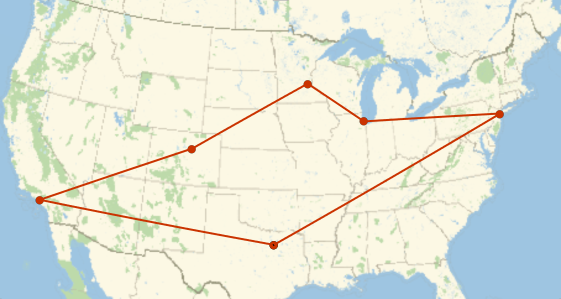
\includegraphics[scale=0.6]{\CURPATH/map1.png}
\caption{}
\end{figure}

Maximizing:

\begin{lstlisting}
sat
Dallas (862 mi to the next city) ->
Minneapolis (700 mi to the next city) ->
Denver (1631 mi to the next city) ->
New York (2451 mi to the next city) ->
Los Angeles (1745 mi to the next city) ->
Chicago (803 mi to the next city) ->
distance_total= 8192 mi
\end{lstlisting}

The map:

\begin{figure}[H]
\centering
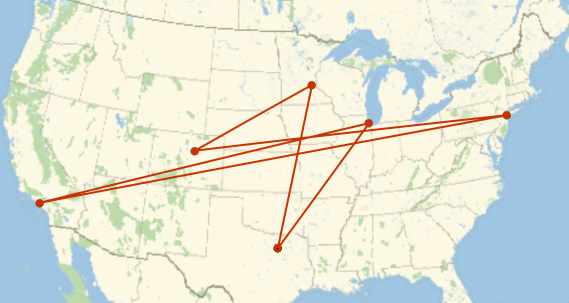
\includegraphics[scale=0.6]{\CURPATH/map2.png}
\caption{}
\end{figure}

I could only process 6 cities, and it takes starting at several seconds up to 1 minute on my venerable Intel Quad-Core Xeon E3-1220 3.10GHz.
Perhaps, this is not a right tool for the job, well-known TSP algorithms way faster.

Even bruteforce enumeration is way faster ($6!=720$ paths).

However, it still can serve as demonstration.

